\section{Software}
Die Steuerung der Segel soll durch zwei verteilte Systeme erfolgen, die über eine Ethernet-Verbindung miteinander kommunizieren. Die Idee dahinter ist, die Berechnungen für die Ausrichtung der Segel in Abhängigkeit der Windstärke und -Richtung (Controllino) von der hardwarenahen Verarbeitung der Sensoren und Aktuatoren (STM32) logisch zu trennen. \\

\noindent
Die vorliegende Arbeit konzentriert sich dabei lediglich auf das System der Sensoren und Aktuatoren, welches mit dem STM32 realisiert wurde. Die Aufgabe dieses Systems ist, zunächst die Linearführung zu kalibrieren, damit die aktuelle Position korrekt ermittelt werden kann. Außerdem soll über die Buttons am Gehäuse und zusätzlich über einen Webserver eine manuelle Steuerung ermöglicht werden. Während des Automatikbetriebs geschieht ein regelmäßiger Austausch aller relevanter Daten über eine REST basierte Schnittstelle. Dies beinhaltet u.A. die Information über aktuelle Windbedingung, Position der Segel, eventuelle Fehlerzustände (z.B. Motorfehler oder Überstrom) und daraus resultierende Befehle zur Anpassung der Segelstellung.
Für die Implementierung wurde die Software in komponentenorientierte Module eingeteilt:
\begin{figure}[H]
	\centering
	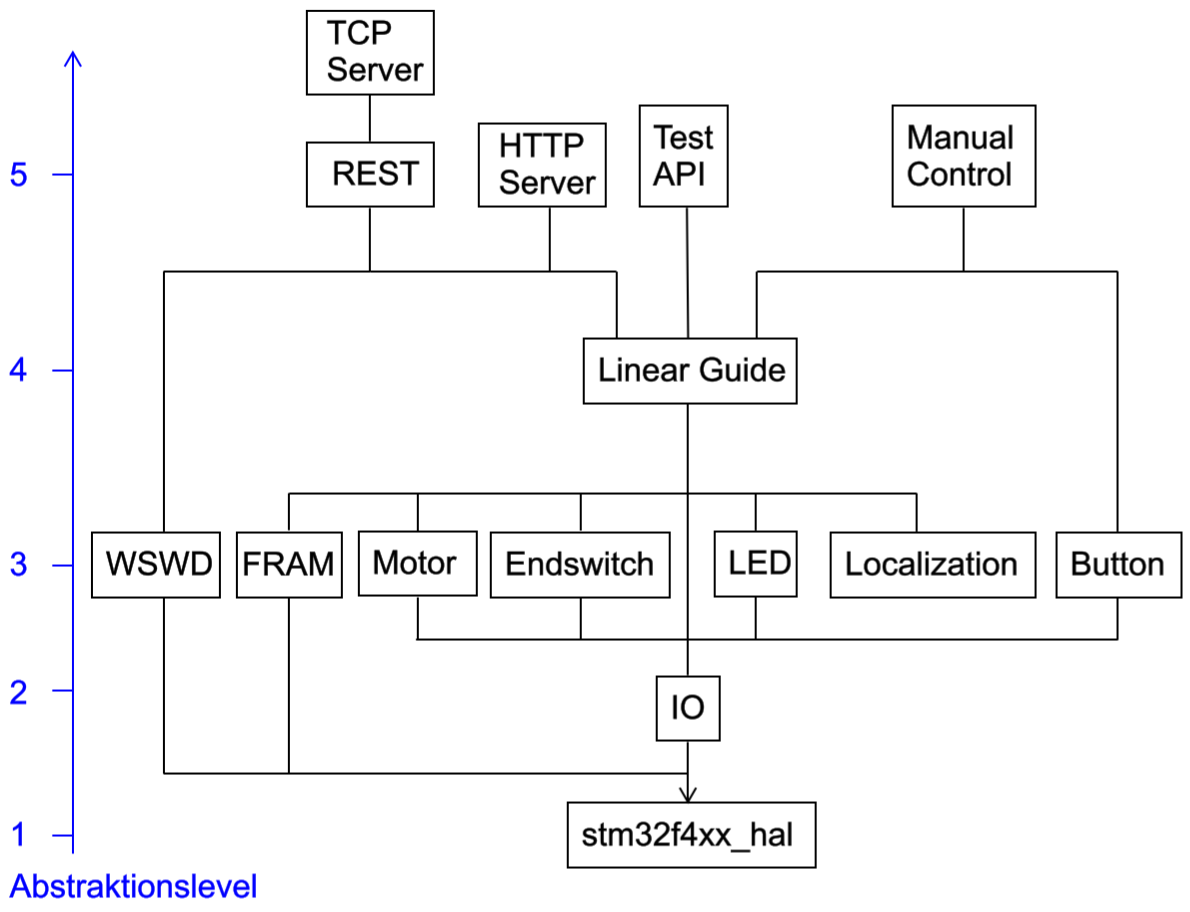
\includegraphics[width=0.6\linewidth]{images/Software/Modulestructure.png}
	\caption{Software Modulstruktur}
	\label{fig:modulestructure}
\end{figure}
\noindent
\autoref{fig:modulestructure} zeigt abwärtsgerichtet, wie die einzelnen Module aufeinander zugreifen. Auf unterster Abstraktionsebene laufen jegliche Operationen über die Standardbibliothek des Mikrocontrollers \verb|stm32f4xx\_hal|. Darüber liefert das \verb|IO|-Modul ein Set aus Hilfsfunktionen und -Strukturen für den allgemeinen Zugriff auf die GPIO-Pins und zum Auslesen analoger Messwerte der einzelnen Sensoren.\\

\noindent
Ebene drei umfasst hauptsächlich Module, welche alle relevanten Funktionalitäten der physischen Teilkomponenten des Systems implementieren, wie z.B. das Anemometer \verb|WSWD| oder der \verb|Motor|. Einige davon greifen dabei auf das \verb|IO|-Modul zu, wobei der allgemeine GPIO-Zugriff von einer spezifischen Funktion eingekapselt wird, wie z.B. das Einschalten einer LED im Falle des \verb|LED|-Moduls. Eine Ausnahme ist das \verb|Localization|-Modul, welches keine physische Komponente darstellt, sondern einige Hilfsfunktionen zur Kalibrierung und Positionsberechnung bereitstellt.\\

\noindent
Während die Module bis Ebene drei überwiegend allgemeingültig entworfen sind, enthält das \verb|Linear Guide|-Modul anwendungsspezifische Funktionen. Als zentrales Element bildet dieses ein High-Level Interface zur Verwendung der Teilkomponenten \verb|FRAM|, \verb|Motor|, \verb|Endswitch|, \verb|LED|, \verb|Localization| und \verb|IO|. \\

\noindent
Die Module der obersten Abstraktionsebene bilden die direkten Schnittstellen zur Außenwelt. Das \verb|Manual Control|-Modul ermöglicht die manuelle Steuerung der Linearführung über die User-Buttons am Gehäuse und insbesondere die Umsetzung des Kalibrierungsprozesses. Auf der anderen Seite kann das System auch durch einen HTTP Webserver überwacht und gesteuert werden. Außerdem werden im \verb|REST|-Modul die Anfragen des Controllinos über die \verb|TCP Server|-Verbindung verarbeitet, wie bereits oben erwähnt. Zuletzt wurde ein \verb|Test|-Modul implementiert, dass die Funktionalitäten der Module auf Ebene drei verifiziert. Dazu wurde ein einfaches Batch-Skript geschrieben, das die einzelnen Testcases auflistet und die Auswahl über UART an den  Mikrocontroller sendet, sodass im \verb|Test|-Modul eine entsprechende Funktion ausgeführt wird. In den nachfolgenden Abschnitten wird genauer auf einige Module eingegangen, beginnend mit dem untersten Abstraktionslevel.

\subsection{IO-Modul}
Dieses Modul soll den lesenden und schreibenden Zugriff auf jegliche GPIO-Pins erleichtern, die zur Kontrolle jeglicher Steuerelemente angeschlossen wurden. Allgemein besteht das System aus analogen und digitalen Sensoren bzw. Aktuatoren. Für jede Form wurde eine repräsentative Struktur definiert, in der alle relevanten Daten zusammengefasst werden.
\subsubsection{Digitale Pins}
Für digitale Ein- und Ausgänge wurde eine gemeinsame Struktur \verb|IO_digitalPin_t| definiert:
\begin{lstlisting}[language=C, caption={Struktur für digitale Pins}, label={lst:digitalPin}]
typedef struct {
	GPIO_TypeDef *GPIOx;
	uint16_t GPIO_Pin;
	GPIO_PinState state;
} IO_digitalPin_t;
\end{lstlisting}
Dabei ist der GPIO-Pin durch eine Nummer \verb|GPIO_Pin| und einen Port \verb|GPIOx| definiert. Zusätzlich wird in der Struktur der aktuelle Zustand \verb|state| (null oder eins) gespeichert. Diese kann nun einer Funktion als Pointer übergeben werden, um z.B. den neuen Zustand auszulesen:
\begin{lstlisting}[language=C, caption={Einlesen eines digitalen Pin-Zustands}, label={lst:digitalRead}]
GPIO_PinState IO_digitalRead(IO_digitalPin_t *dig_IN) {
	dig_IN->state = HAL_GPIO_ReadPin(
		dig_IN->GPIOx, dig_IN->GPIO_Pin
	);
	return dig_IN->state;
}
\end{lstlisting}
Dabei wird lediglich die Funktion \verb|HAL_GPIO_ReadPin()| der \verb|stm32f4xx_hal| Bibliothek aus \autoref{fig:modulestructure} aufgerufen, welche die zuvor besagten Attribute des Pins entgegennimmt und dessen Wert zurückgibt. Das Speichern dieses Werts in \verb|state| hat den Vorteil, dass damit auf eine Änderung des Zustandes geschlossen werden kann. Dies ist z.B. für das Erfassen der steigenden und fallenden Flanke während eines Knopfdrucks sinnvoll und wurde wie folgt realisiert:
\begin{lstlisting}[language=C, caption={Detektion einer Flanke}, label={lst:edgeDetection}]
boolean_t IO_digitalRead_state_changed(IO_digitalPin_t *dig_IN) {
	GPIO_PinState previous_state = dig_IN->state;
	GPIO_PinState current_state = IO_digitalRead(dig_IN);
	return current_state ^ previous_state;
}
\end{lstlisting}
Die Funktion in \autoref{lst:edgeDetection} gibt durch eine logische exklusiv-oder-Verknüpfung von letztem und aktuellem Zustand in Form eines booleschen Werts an, ob sich der Zustand geändert hat oder nicht. Äquivalent zu \autoref{lst:digitalRead} ist eine Funktion \verb|IO_digital_write()| implementiert, die den gewünschten Pegel an einem entsprechenden Ausgangspin schaltet.
\subsubsection{Analoge Pins}
Etwas komplexer wird es mit dem Auslesen von analogen Sensorwerten. Dazu wird ein ADC-Kanal (\verb|ACD_Channel|) des STM32 verwendet, der eine Spannung am Pin zwischen 0 und 3.3V in eine 12 bit Sequenz quantisiert und folglich als Integerwert \verb|ADC_val| zwischen 0 und 4096-1 zurückgibt. Idealerweise entspricht dieser Wertebereich umgewandelt dem des Sensors, jedoch ist dies durch Ungenauigkeiten in der Hardware nicht immer der Fall, weshalb dies durch zusätzliche Grenzwerte in der Struktur für analoge Sensoren berücksichtigt wird:
\begin{lstlisting}[language=C, caption={Struktur für analoge Sensoren}, label={lst:analogSensor}]
typedef struct {
	ADC_HandleTypeDef *hadc_ptr;
	IO_SensorType_t Sensor_type;
	uint32_t ADC_Channel;
	uint16_t ADC_val;
	uint16_t max_sens_val;
	uint16_t sens_val;
	uint16_t min_sens_val;
	float max_pin_volt;
	float min_pin_volt;
} IO_analogSensor_t;
\end{lstlisting}
Die Bezeichnung \verb|sense_val| aus \autoref{lst:analogSensor} steht dabei für den Wert in der Einheit des gewünschten Sensormesswerts und \verb|pin_volt| für den umgewandelten Spannungswert am Pin. Damit lässt sich der Sensormesswert wie folgt berechnen:\footnote{Funktion dient zur Veranschaulichung und wurde nicht exakt in dieser Form implementiert}
\begin{lstlisting}[language=C, caption={Konvertierung des rohen Analogwerts}, label={analogRead}]
void IO_Convert_from_ADC(IO_analogSensor_t *s) {
	float pin_volt = 3.3 * s->ADC_val / (4096-1)
	s->sens_val = (s->max_sens_val - s->min_sens_val) /
	              (s->max_pin_volt - s->min_pin_volt) *
	              (pin_volt        - s->min_pin_volt) +
	               s->min_sens_val
}
\end{lstlisting}
In umgekehrter Weise funktioniert die Umwandlung eines gewünschten Wertes in einen quantisierten Spannungswert für einen analogen Aktuator mithilfe einer entsprechenden Struktur \verb|IO_analogActuator_t|. \\

\noindent
Die Module \verb|LED|, \verb|Button| und \verb|Endswitch|, repräsentieren physische Komponenten, die jeweils durch einen einfachen digitalen Pin angesteuert werden und enthalten daher lediglich Wiederverwendungen der Funktionen \verb|IO_digitalWrite()|, um eine LED ein und auszuschalten, \verb|IO_digitalRead_state_changed()|, um einen Knopfdruck zu erfassen oder \verb|IO_digitalRead()|, um den Zustand eines Endschalters zu lesen. Dagegen wird der BG 45x30 SI Gleichstrommotor aufgrund seiner internen Regelung durch mehrere verschiedene Ein- und Ausgänge angesteuert.
\subsection{Motor-Modul}
Die Aufgabe des Motors ist, die Segelstellung entlang der Linearführung anzupassen. Dazu ermöglichen dessen digitale Eingänge gemäß \autoref{tab:digitale_Eingaenge} eine flexible Einstellung der Drehzahl und -Richtung. Alternativ zu den konfigurierbaren fixen Geschwindigkeiten 1 und 2 kann mit dem analogen Eingang auch eine beliebige Drehzahl dynamisch vorgeben werden. Damit konnte eine Drehzahlrampe realisiert werden, die einen sanfteren Brems- und Beschleunigungsvorgang gewährleistet.\\

\noindent
Über die digitalen Ausgänge kann der Ist-Zustand überwacht werden, darunter die aktuelle Drehrichtung und ob ein Fehler vorliegt. Zusätzlich kann durch ein Puls-Signal mit 12 Pulsen pro Umdrehung auf die Drehzahl geschlossen werden. Da der Motor in diesem Fall jedoch unter Drehzahlregelung betrieben wird, kann, sofern kein Fehlersignal vorliegt, von einer ausreichend präzisen Einhaltung der eingestellten Drehzahl ausgegangen werden. Dennoch ist das Puls-Signal von zentraler Bedeutung, da aufgrund der Gewindesteigung der Linearführung und der Anzahl der Pulse ausgehend von einem Endpunkt die aktuelle Position und somit die Segelstellung ermittelt werden kann. Das Zählen der Pulse geschieht jedoch der Thematik entsprechend in einer Funktion des \verb|Localization|-Moduls, die durch einen externen Interrupt am zuständigen GPIO-Pin von steigenden Flanken getriggert wird.\\

\noindent
Orientiert an der Architektur des \verb|IO|-Moduls dient auch hier eine Struktur als gemeinsamer Zugriffspunkt aller relevanter Daten des Motors:
\begin{lstlisting}[language=C, caption={Struktur des Motors}, label={lst:motor}]
typedef struct {
	Motor_function_t current_function;
	Motor_INs_t INs;
	IO_analogActuator_t AIN_set_rpm;
	IO_digitalPin_t OUT2_error;
	IO_digitalPin_t OUT3_rot_dir;
	uint16_t normal_rpm;
	uint16_t rpm_set_point;
	uint16_t ramp_final_rpm;
	uint32_t ramp_last_step_ms;
	boolean_t ramp_activated;
} Motor_t;
\end{lstlisting}
\subsubsection{Funktionsvorgabe}
Grundlage zur Steuerung des Motors ist die Implementation der Funktionsvorgabe über die digitalen Eingänge, die in der Struktur nach \autoref{lst:motor} durch ein Array \verb|INs| des Typs \verb|IO_digitalPin_t| organisiert sind. Zur einfachen Anwendung wurde ein enum \verb|Motor_function_t| definiert, der alle Funktionen entsprechend \autoref{tab:digitale_Eingaenge} bezeichnet und von oben beginnend von null bis sieben nummeriert. Durch eine geeignete Umrechnung in einen Binärwert zwischen 00 und 11 können aus den einzelnen Stellen direkt die passenden beiden Pins über das Array indiziert und mit den Stellenwerten beschrieben werden. Das nachfolgende Listing zeigt die genaue Umsetzung dieses Verfahrens.
\begin{lstlisting}[language=C, caption={Einstellung der Motorfunktionen}, label={lst:motorFunction}]
void Motor_set_function(Motor_t *motor, Motor_function_t func) {
	motor->current_function = func;
	uint8_t pin_offset = (func >= 4) * 2;
	int8_t function_bits = func - pin_offset * 2;
	for (int i = 0; i < 2; i++) {
		GPIO_PinState state = function_bits & 2 ? 1 : 0;
		uint8_t IN_idx = i + pin_offset;
		IO_digitalWrite(&motor->INs[IN_idx], state);
		function_bits <<= 1;
	}
}
\end{lstlisting}
Im ersten Schritt wird überprüft, ob die Eingänge 0 \& 1 oder 2 \& 3 für die Funktion zuständig ist. Letzteres ist der Fall, wenn der Funktionsindex in der oberen Hälfte (\verb|>=4|) liegt. Das Beschreiben der beiden Eingänge erfolgt iterativ über eine For-Schleife, wobei die Pins durch die Zählvariable \verb|i| indiziert werden. Falls die Eingänge 2 \& 3 zuständig sind, muss folglich ein \verb|pin_offset| von zwei auf den Index addiert werden. Ebenfalls wird dann die Funktionsnummer mit vier subtrahiert, damit aus dem resultierenden Wert in \verb|function_bits| der zweistellige Binärwert errechnet werden kann.
Durch die bitweise und-Verknüpfung mit zwei und einer anschließenden einfachen links-shift Operation (\acs{MSB}-first) werden die einzelnen Binärstellen der Reihe nach berechnet und mit \verb|IO_digitalWrite()| als neuen Zustand \verb|state| am passenden Pin geschaltet.
\subsubsection{Drehzahlrampe}
Darauf basierend wurden konkrete Funktionen zur Steuerung des Motors implementiert. Das Kernelement ist dabei die Realisierung der Drehzahlrampe innerhalb der Funktion \verb|Motor_speed_ramp()|, welche in der Hauptschleife des Programms durchgehend ausgeführt wird. Die Rampe kann dabei durch eine Funktion \verb|Motor_start_moving()| aktiviert werden, die mit \verb|Motor_set_function()| Links- oder Rechtslauf einstellt und anschließend das Flag \verb|ramp_activated| aus \autoref{lst:motor} setzt. Darauf hin wird der Drehzahlwert \verb|rpm_setpoint| in regelmäßigen Zeitschritten um einen konstanten Wert erhöht. Nach Konfiguration auf \textit{Drehzahlvorgabe} (\autoref{tab:digitale_Eingaenge}) kann die neue Soll-Drehzahl an dem analogen Eingang \verb|AIN_set_rpm| mit \verb|IO_analogWrite()| umgesetzt werden. Dies geschieht solange, bis die Zieldrehzahl \verb|ramp_final_rpm=normal_rpm| erreicht ist und die Rampe wieder deaktiviert wird. Ebenso kann die Rampe mit \verb|Motor_stop_moving()| für den Bremsvorgang aktiviert werden, wobei \verb|ramp_final_rpm=0| gesetzt wird und die Drehzahl in gleicher Weise schrittweise reduziert wird. Aufgrund einiger Tests wurde für die Rampe eine Schrittdauer von 13 ms und eine Schrittweite von 10 rpm mit einer Normaldrehzahl von 1600 rpm festgelegt, sodass sich folgender zeitlicher Verlauf ergibt:
\begin{figure}[H]
	\centering
	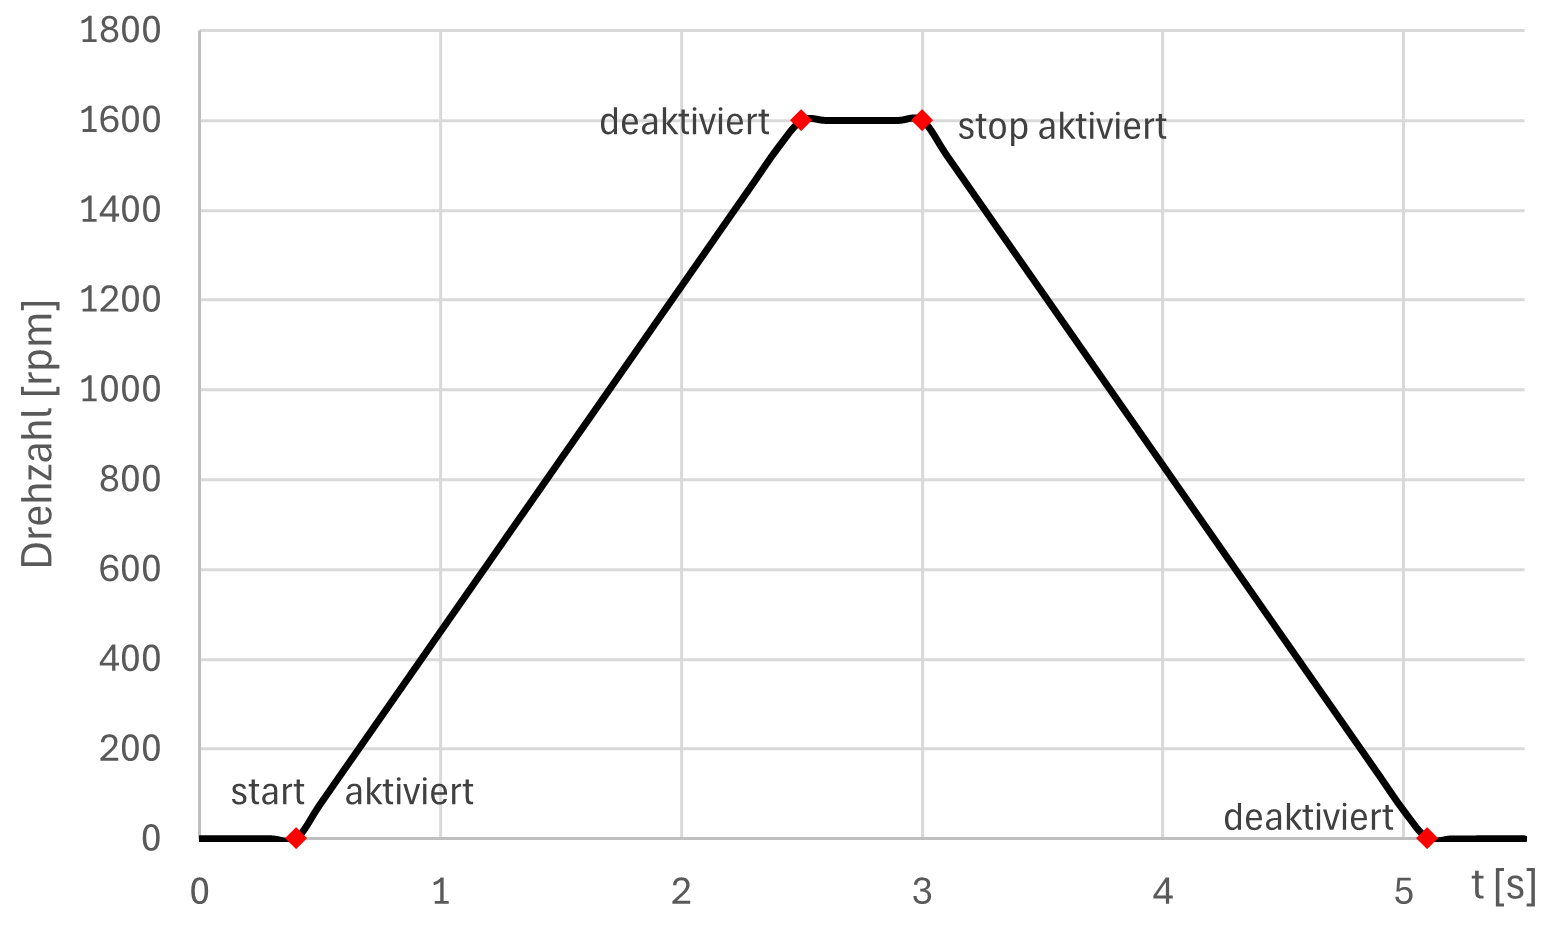
\includegraphics[width=0.75\linewidth]{images/Software/SpeedRamp.png}
	\caption{Drehzahlrampe: Beschleunigen und Bremsen}
	\label{fig:speedRamp}
\end{figure}
\noindent
Die Stopp-Funktion bietet zusätzlich die Möglichkeit über einen booleschen Parameter \verb|immediate| z.B. während einer Notabschaltung den Motor abrupt anzuhalten. In diesem Fall wird nicht die Rampe aktiviert sondern direkt die Motorfunktion \textit{Motor aus} gesetzt. 
\subsection{Steuerung der Linearführung}
nachdem die allgemeine Steuerung des Motors implementiert ist, gilt es, diese auf die Positionierung der Segel über die Linearführung anzuwenden. 
\subsubsection{Kalibrierung}\label{subsubsec:Kalibrierung}
Damit später eine bestimmte Stellung angefahren werden kann, muss die aktuelle Position jederzeit bekannt sein. Wie bereits erwähnt, dient das Puls-Signal des Motors als Maß, wie weit sich die Position von einem Startpunkt entfernt hat. Jedoch muss dieser Punkt erst angefahren werden, was durch die Detektion der Endschalter keine Schwierigkeit darstellt. Damit kann die absolute Position anhand der Puls-Zahl und der Gewindesteigung ermittelt werden. Für die Einstellung der Segel wird vom Controllino eine Prozentzahl vorgegeben wie weit gerollt oder getrimmt werden soll. Um diesen Wert auf eine absolute Position auf der Linearführung abzubilden, muss zusätzlich die Distanz zwischen den beiden Endpunkten ermittelt werden. Außerdem soll die Grenze zwischen Roll- und Trimmbereich nachträglich manuell angepasst werden können, um potenzielle Asymmetrien in der Seilführung der Segel auszugleichen. Der gesamte Ablauf der Kalibrierung wurde in Form einer Zustandsmaschine realisiert, wie in \autoref{fig:calibration} dargestellt.
\begin{figure}[H]
	\centering
	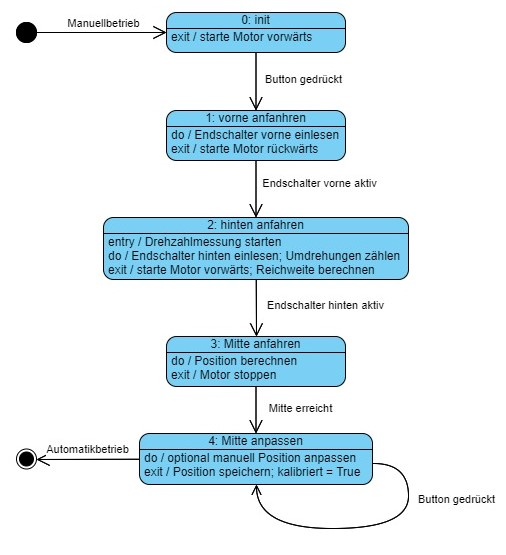
\includegraphics[width=0.8\linewidth]{images/Software/Kalibrierungsprozess.jpg}
	\caption{Kalibrierungsprozess}
	\label{fig:calibration}
\end{figure}
\noindent
Die Eintrittsbedingung der Kalibrierung ist das Einschalten des manuellen Betriebsmodus durch den Kippschalter am Gehäuse oder alternativ über den Webserver. Aus dem Ausgangszustand heraus muss der Knopf \textit{Speichern/Bestätigen} aus \autoref{fig:Bedienung} gedrückt werden, um die automatische Kalibrierung einzuleiten. Dies ist mit dem starten des Motors in Vorwärtsrichtung und dem Übergang in Zustand 1 verbunden. Anschließend wird der vordere Endschalter abgefragt, bis dieser aktiviert wird und die Endposition erreicht ist. Von dieser Position aus beginnt die Pulszählung, damit nach Ankunft am anderen Ende die zurückgelegte Distanz berechnet werden kann. Aus dieser Distanz wird daraufhin die Mitte bestimmt und angefahren. Ist diese erreicht, kann zuletzt die tatsächliche Grenze manuell über die Knöpfe \textit{Trimmen} und \textit{Rollen} angefahren und mit dem erneuten Druck des einleitenden Knopfes bestätigt werden. Als Feedback blinkt dabei die LED \textit{Position gespeichert}. Ebenso aktivieren bzw. deaktivieren sich nun nach der Einteilung der Bereiche je nach Positionierung die entsprechenden LEDs (\textit{Im Trimmungsbereich} / \textit{Im Rollbereich}).\\

\noindent
Da die Grenze in Zustand 4 mit dem entsprechenden Knopf beliebig oft angepasst werden kann, ist es durch das selbe Signal nicht möglich, den kompletten Prozess von vorne zu starten, ohne das System neu zu booten. Daher wurde ein Timer mit einem periodischen Callback konfiguriert, der die Dauer des Knopfdrucks ermittelt und ab einer Druckdauer von 3s die Zustandsmaschine zurücksetzt, anstatt lediglich die Grenze zu überschreiben. Nach Abschluss der Kalibrierung kann in den Automatikbetrieb gewechselt werden, indem der Controllino aufgrund der bereitgestellten Daten regelmäßig die optimale Segelstellung neu berechnet und an den stm32 zurückgibt. Der nächste Abschnitt beschäftigt sich damit, wie genau die gewünschte Segelstellung in eine Position auf der Linearführung umgerechnet wird. 
\subsubsection{Umsetzung einer Rollung/Trimmung}
Der Befehl einer Segelanpassung wird vom Controllino durch einen Modus (Rollen oder Trimmen) und eine Prozentzahl definiert. \autoref{fig:linearGuide} zeigt graphisch die Bedeutung dieser Angabe bezüglich der Positionierung an der Linearführung.
\begin{figure}[H]
	\centering
	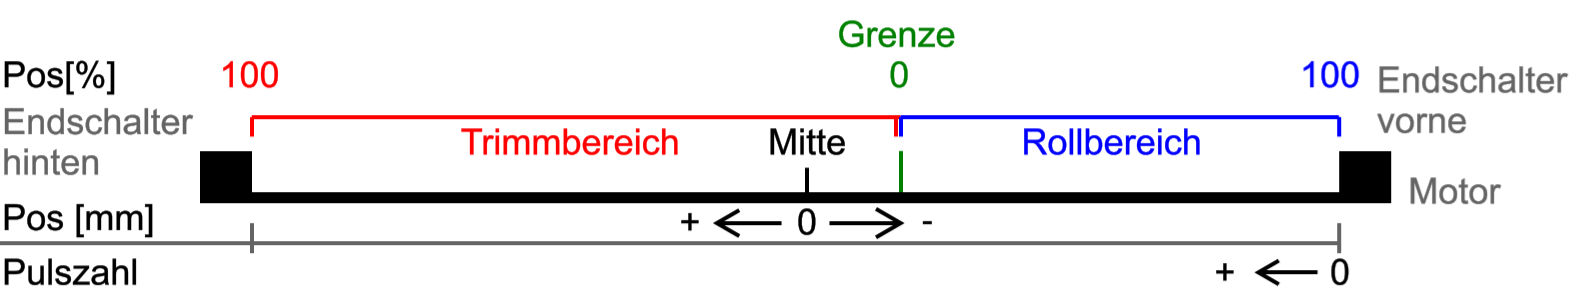
\includegraphics[width=\linewidth]{images/Software/LinearGuide.png}
	\caption{Rollung und Trimmung an der Linearführung}
	\label{fig:linearGuide}
\end{figure}
\noindent
In diesem Beispiel weicht die Grenze zwischen den beiden Bereichen stark von der tatsächlichen Mitte ab, um die Möglichkeit deren manuellen Anpassung, wie zuvor erwähnt zu verdeutlichen. Zur besseren Lesbarkeit der aktuellen Position wird diese in einem Zwischenschritt in mm umgerechnet und die Mitte der Gesamtdistanz auf null zentriert. In dieser Einheit werden jegliche Positionsberechnungen durchgeführt. \\

\noindent
Für die Umwandlungen zwischen Prozent, mm und Pulsen werden alle relevanten Daten in einer gleichnamigen Struktur des \verb|Localization|-Moduls festgehalten. \autoref{lst:sailAdjustment} zeigt die Ermittlung der gewünschten Position in mm mithilfe dieser Struktur aufgrund eines Segelanpassungsbefehls:
\begin{lstlisting}[language=C, caption={Berechnung der Zielposition}, label={lst:sailAdjustment}]
void Linear_Guide_set_desired_roll_trim_percentage(
	Localization_t *loc, uint8_t percentage, 
	adjustment_mode_t mode
)
{
	int8_t sign = mode == adjustment_mode_roll ? 1 : -1;
	int32_t roll_trim_distance = loc->end_pos_mm
	                           + sign * loc->center_pos_mm;
	loc->desired_pos_mm = (int32_t) 
	(- sign * (roll_trim_distance * (percentage / 100.0F)
	           - sign * loc->center_pos_mm));
}
\end{lstlisting}
Zunächst wird ein Vorzeichen \verb|sign| festgelegt, da der Rollbereich im negativen und der Trimmbereich im positiven mm Bereich liegt. Je nachdem welche Modus gewünscht ist, berechnet sich dessen Streckenanteil an der Linearführung aus der Distanz \verb|end_pos_mm| von der Mitte bis zu einem Endpunkt und dem Abstand \verb|center_pos_mm * sign| von der Mitte bis zur gewählten Grenze \verb|center_pos_mm|. Von dieser Strecke wird der gewünschte Anteil \verb|percentage| durch das Vorzeichen auf die richtige Seite orientiert. Zuletzt muss das addieren des Abstandes \verb|center_pos_mm * sign| wieder rückgängig gemacht werden.\\

\noindent
Nachdem die gewünschte Position in mm vorliegt, muss diese angesteuert werden. Dazu muss diese mit der aktuellen Position der Linearführung verglichen werden, welche sich nach der Kalibrierung aus der Pulszahl des Motors ergibt. Die Pulszahl wird wie bereits erwähnt durch den externen Interrupt am zuständigen GPIO-Pin regelmäßig aktualisiert und in der Struktur \verb|Localization_t| aus \autoref{lst:sailAdjustment} festgehalten. Die Positionsumrechnung ist in einer Funktion des \verb|Localization|-Moduls implementiert, wie nachfolgend gezeigt:
\begin{lstlisting}[language=C, caption={Positionsberechnung aus dem Pulssignal des Motors}, label={lst:pulseToPos}]
void Localization_update_position(Localization_t *loc)
{
	uint16_t abs_pos = loc->pulse_count
	                 * loc->distance_per_pulse;
	loc->current_pos_mm = abs_pos - loc->end_pos_mm;
}
\end{lstlisting}
Dabei berechnet sich die zurückgelegte Strecke pro Puls \verb|distance_per_pulse| aus dem Quotienten der Gewindesteigung von 1.12 mm pro Umdrehung und der Pulsfrequenz des Motors von 12 Pulsen pro Umdrehung zu 0.093 mm pro Puls.
\subsubsection{Optimierung der Bewegungsübergänge}
Die Steuerung der Linearführung wird durch das Aktivieren von Drehzahlrampen gelöst, um sanfte Beschleunigungs- und Bremsvorgänge zu ermöglichen. Allerdings gibt es unter dem bisherigen Stand der Implementierung mehrere Situationen, in denen es trotzdem noch zu abrupten Bewegungsänderungen kommt. Eine davon stellt das Erreichen eines Endpunktes dar, denn die Aktivierung des Endschalters ist direkt mit einem hardware-geregelten Stopp des Motors verbunden. Ebenfalls kann die Rampenfunktion nicht zwischen Beschleunigung in Vorwärts- und Rückwärtsrichtung unterscheiden, weshalb bei ein Befehl in die umgekehrte Richtung sofort umgesetzt wird. Ein anderes vielleicht noch wichtigeres Problem ist, dass eine gewünschte Position nicht korrekt angefahren werden kann, da der Motor nach dem Stopp-Befehl aufgrund der Rampe noch ein kleines Stück weiterfährt.\\

\noindent
Die Lösung dieser Probleme liegt in der Ermittlung des Bremsweges sowie der Einführung einer Warteschlange für Zielpositionen. Darauf basierend wurde ein Algorithmus zur optimierten Koordination der Steuerbefehle implementiert, wie nachfolgend in Form eines Programmablaufplans dargestellt:
\begin{figure}[H]
	\centering
	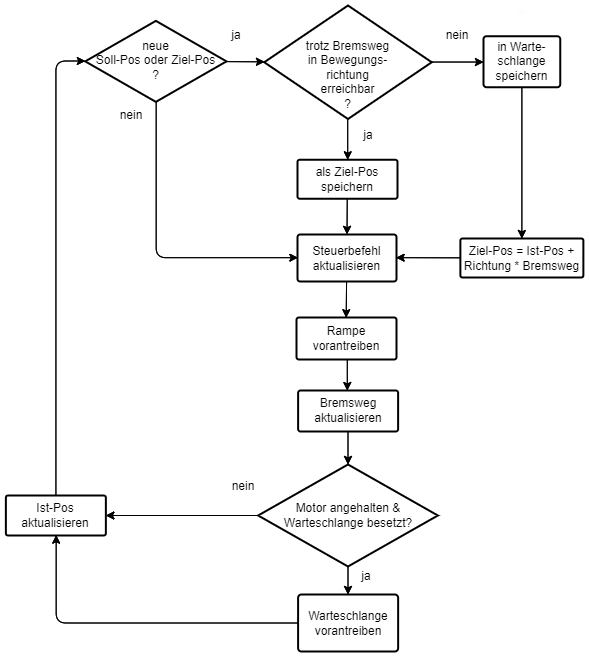
\includegraphics[width=\linewidth]{images/Software/ControlOptimization.png}
	\caption{Optimierung der Steuerbefehle}
	\label{fig:controlOptimization}
\end{figure}
\noindent
Eine Soll-Position kann entweder durch die manuelle Steuerung oder durch eine gewünschte Segelstellung vom Controllino während des Automatikbetriebs vorgegeben werden. Hat sich diese geändert, kann es sein, dass sich die Linearführung wegen eines vorhergegangenen Befehls bereits in Bewegung befindet. In diesem Fall muss überprüft werden, ob sich die Soll-Position in Bewegungsrichtung vor der aktuellen Position befindet und ggfs. ob der Abstand aufgrund des Bremsweges noch erreichbar ist. Wenn diese Bedingungen nicht erfüllt sind, wird die Soll-Position nicht direkt als neues Ziel gesetzt sondern in einer Warteschlange gespeichert, wobei diese eigentlich nur eine einzelne Variable der \verb|Localization_t| Struktur ist. Damit die neue Soll-Position trotzdem so schnell wie möglich erreicht wird, bildet der in Fahrtrichtung nächste noch erreichbare Punkt die neue Zielposition. Danach kann der Steuerbefehl aktualisiert werden (Vorwärts, Rückwärts oder anhalten). Nach Vorantreiben der Rampe muss der Bremsweg aufgrund der aktuellen Drehzahl ebenfalls neu berechnet werden. Ist der Motor zum Stillstand gekommen, kann sofern vorliegend die Position aus der Warteschlange als neues Ziel vorgerückt werden. Zuletzt muss natürlich auch die aktuelle Position der Linearführung aktualisiert werden bevor der Kreislauf von neuem beginnt. \\

\noindent
Sollte eine Soll-Position auch nach einem Richtungswechsel aufgrund einer Fehlberechnung des Bremsweges verfehlt werden, wird diese einfach erneut in die Warteschlange gesetzt, sodass sich die exakte Position garantiert einpendelt. Zusammenfassend werden nun mithilfe der Ziel-Warteschlange abrupte Richtungswechsel vermieden und durch die Berechnung des Bremsweges kann das System rechtzeitig anhalten, um die Soll-Position präzise anzufahren oder den Aufprall am Endschalter zu verhindern.
\subsubsection{Wiederherstellung der Position}
Die in Kapitel \ref{subsubsec:Kalibrierung} beschriebene Kalibrierung ist ein zeitintensiver Prozess. Damit diese nicht bei jedem Programmneustart erneut durchgeführt werden muss, wurde ein FRAM Speicher in der Hardware verbaut, um dort alle relevanten Informationen zur Wiederherstellung der aktuellen Position hineinzuschreiben und bei Bedarf wieder auszulesen. Für diese beiden Funktionen wurde ein Benutzerinterface im \verb|FRAM|-Modul implementiert.\\

\noindent
Das \ac{FRAM} Modul steuert den \ac{FRAM} über \ac{SPI} an. Der FRAM kann dabei über sechs Befehle gesteuert werden. Dabei wurden die Befehle: WREN(0000 0110b), RDSR(0000 0101b), READ(0000 0011b) und WRITE(0000 0010b) genutzt. Um auf den Speicher zu schreiben wird das \ac{WREN} Bit gesetzt. Hierfür wird der gleichnamige Befehl genutzt. Um zu überprüfen ob das Bit gesetzt wurde, wird mit dem Befehl RDSR das Status Register ausgelesen und das Bit 7 überprüft. Um auf den Speicher zu schreiben wird mit dem WRITE Befehl gefolgt von einer 12Bit Addresse der Speicherbereich ausgewählt. Die Darauffolgenden Bits werden in den Speicher geschrieben. Beim auslesen mit dem Befehl READ ist das vorgehen gleich, nur werden hier keine zusätzlichen Bits übertragen. In der Software wurden dabei die zwei Funktionen \verb|FRAM_write| und \verb|FRAM_read| erstellt die für einen high level access sorgen. Über diese kann ein Puffer in den \ac{FRAM} geschrieben werden oder die Daten ausgelesen werden. Die Serialisierung und Deserialisierung, sowie das setzen des \ac{WREN} Bits wird beim Aufruf übernommen.\\

\noindent
Damit die Daten beim Auslesen zur Initialisierung des Systems aktuell sind, werden diese bei jeder Positionsänderung an der entsprechenden Speicheraddresse überschrieben. Die für die Lokalisierung nötigen Informationen werden zur Serialisierung innerhalb einer separaten Struktur organisiert, wie nachfolgend gezeigt:
\begin{lstlisting}[language=C, caption={Speicherformat der Positionsdaten}, label={lst:locSafeData}]
typedef struct {
	Loc_state_t state;
	int16_t pulse_count;
	uint16_t end_pos_mm;
	int16_t center_pos_mm;
	uint16_t start_pos_abs_mm;
} Loc_safe_data_t;
\end{lstlisting}
Die bisher nicht eingeführte Variable \verb|start_pos_abs_mm| entspricht dem vom Distanzsensor gemessenen Abstand der Position bei Aktivierung des vorderen, motor-seitigen Endschalters. Daraus lässt sich die mit dem Puls-Signal ermittelte Position mit dem Messwert des Sensors vergleichen. Die Bedeutung der Messung wird in Kapitel \ref{subsubsec:Fehlerbehandlung} genauer behandelt. \\

\noindent
Der Schreibprozess dieser Daten in das FRAM ist durch eine Funktion \\\verb|Linear_Guide_safe_Localization()| gegeben. \autoref{lst:safeLocalization} zeigt deren Implementierung.
\begin{lstlisting}[language=C, caption={FRAM Speichervorgang}, label={lst:safeLocalization}]
int8_t Linear_Guide_safe_Localization(Localization_t loc)
{
	uint8_t FRAM_buffer[sizeof(Loc_safe_data_t)];
	Localization_serialize(loc, FRAM_buffer);
	if(FRAM_write(FRAM_buffer, 
	              LINEAR_GUIDE_INFOS, 
	              sizeof(Loc_safe_data_t)) != HAL_OK)
	{
		printf("Saving Position failed!\r\n");
		return LG_LOCALIZATION_FAILED;
	}
	return LG_LOCALIZATION_SAFED;
}
\end{lstlisting}
Zunächst wird ein FRAM-Puffer der Größe des Speicherformats aus \autoref{lst:locSafeData} deklariert. Dann werden die entsprechenden Daten in der Funktion\\ \verb|Localization_serialize()| von der Struktur \verb|loc| in das richtige Format extrahiert und anschließend an den Puffer adressiert. Zuletzt werden die Daten innerhalb des Puffers durch \verb|FRAM_write()| an die definierte Addresse\\ \verb|LINEAR_GUIDE_INFOS| des physischen Speichers transferiert.\\

\noindent
Nachdem die Daten während des Betriebs kontinuierlich im FRAM aktualisiert werden, können diese bei einem Neustart des Systems in umgekehrter Weise wie in \autoref{lst:safeLocalization} durch \verb|FRAM_read()| abgerufen werden. \autoref{lst:deserialize} zeigt die Verarbeitung des resultierenden Ausgangspuffers \verb|buffer|:
\begin{lstlisting}[language=C, caption={Auslesen der Positionsdaten aus dem FRAM-Puffer}, label={lst:deserialize}]
static int8_t Localization_deserialize(
	Localization_t *loc, 
	uint8_t buffer[sizeof(Loc_safe_data_t)]
)
{
	Loc_safe_data_t *data = (Loc_safe_data_t *)
		malloc(sizeof(Loc_safe_data_t));
	memcpy(data, buffer, sizeof(Loc_safe_data_t));
	loc->state = data->state;
	loc->pulse_count = data->pulse_count;
	loc->end_pos_mm = data->end_pos_mm;
	loc->center_pos_mm = data->center_pos_mm;
	loc->start_pos_abs_mm = data->start_pos_abs_mm;
	free(safe_data_ptr);
	if (loc->state != Loc_state_5_center_pos_set)
	{
		return LOC_RECOVERY_RESET;
	}
	return LOC_RECOVERY_COMPLETE;
}
\end{lstlisting}
Im ersten Schritt wird ein Pointer \verb|data| im Speicherformat \verb|Loc_safe_data_t| entsprechend allokiert, damit diesem anschließend mit der c-Standard-Funktion \verb|memcpy()| die Daten aus dem Puffer übertragen werden können. Danach werden die einzelnen Werte der Reihe nach der Hauptstruktur des \verb|Localization|-Moduls übergeben. Zuletzt wird mit der \verb|state|-Variable überprüft, ob die Kalibrierung beim letzten Betrieb abgeschlossen wurde. Falls nicht, muss diese wiederholt werden, was das Rückgabe-Flag \verb|LOC_RECOVERY_RESET| signalisiert. War die Wiederherstellung der Lokalisierung erfolgreich, kann die aktuelle Position wie gehabt entsprechend \autoref{lst:pulseToPos} mit den Werten \verb|pulse_count| und \verb|end_pos_mm| ermittelt werden. Durch das Speichern der Grenze \verb|center_pos_mm| bleiben außerdem auch die zuvor eingestellten Trimm- und Rollbereiche erhalten.
\subsubsection{Fehlerbehandlung}\label{subsubsec:Fehlerbehandlung}
Mithilfe der Sensoren und dem Fehlersignal des Motors können verschiedene Fehlerzustände identifiziert werden. \autoref{tab:Fehlerbehandlung} listet diese auf, stellt deren Bedingung dar und wie damit umgegangen wird.
\begin{table}[H]
	\centering
	\begin{tabular}{|c|c|c|c|}
		                                                                                    \hline
		\textbf{ID} & \textbf{Bezeichnung} & \textbf{Bedingung}  & \textbf{Behandlung}   \\ \hline
		0           & Normal               & kein Fehler         & keine                 \\
		            &                      & identifiziert       &                       \\ \hline
		1           & Distanzfehler        & Toleranz von 1 cm   & Anpassung an Messwert \\
		            &                      & zwischen Messwert   &                       \\
		            &                      & und Pulsberechnung  &                       \\
		            &                      & überschritten       &                       \\ \hline
		2           & Windfehler           & max. Geschwindigkeit& Segel 100 \% einrollen\\
		            &                      & überschritten       &                       \\ \hline
		3           & Motorfehler          & Fehlersignal aktiv  & Notabschaltung        \\ \hline
		4           & Stromfehler          & Stromsensorwert von & Notabschaltung        \\
		            &                      & 4 A überschritten   &                       \\ \hline
	\end{tabular}%
	\caption{Fehlerzustände}
	\label{tab:Fehlerbehandlung}
\end{table}
\noindent
Bei jedem Fehler leuchtet als Feedback die LED \textit{Störung} aus \autoref{fig:Bedienung} auf. Während Fehler 1 vom System automatisch korrigiert werden kann, wird bei den anderen im Gegensatz dazu der weitere Betrieb solange blockiert, bis diese behoben sind. Die Toleranz zur maximalen Windgeschwindigkeit soll dabei vom Controllino festgelegt werden, da dort auch die Berechnungen zur optimalen Segelstellung durchgeführt werden. Daher wird der Windfehler auch nicht vom STM32 selbst gesetzt, sondern vom Controllino über das REST-Protokoll kommuniziert.
\subsection{Windmessung mit dem Anemometer}
Wie bereits in \autoref{Mangelnde_Präzision} aufgezeigt war die Präzision der Analogen Signale zwar ausreichend aber teilweise sehr ungenau. Aus diesem Grund wurde stattdessen die digitale RS485 Schnittstelle zur Übertragung der Windgeschwindigkeit und Windrichtung genutzt. Der WSWD bietet dabei mehrere Protokolle an, um diese Daten Formattiert zu übertragen. Dabei wurde das \ac{NMEA} Telegramm ausgewählt. Die Formatierung ist in \autoref{fig:NMEA_Protokoll} dargestellt.
\begin{figure}[H]
	\centering
	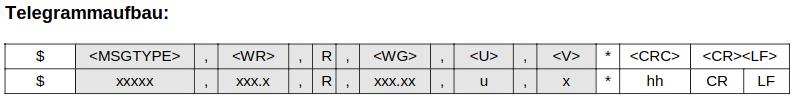
\includegraphics[width=\linewidth]{images/Software/NMEA_Telegramm_Aufbau.png}
	\caption{Aufbau eines NMEA Telegramm (vgl.\cite{WSWD}, S.61)}
	\label{fig:NMEA_Protokoll}
\end{figure}
\noindent Hier wird neben den Daten ($<WR>$ und $<WG>$) ebenfalls die Gültigkeit der Messung ($<V>$) und die Einheit der Geschwindigkeit ($<U>$) übertragen. Das versenden von Befehlen geschieht dabei aber in einem von MESA selbsterstellten Format:
\begin{table}[H]
	\centering
	\begin{tabular}{|l|l|l|l|}
		\hline
		\textbf{\textless{}ID\textgreater{}} & \textbf{\textless{}CM\textgreater{}} & \textbf{\textless{}PARAM\textgreater{}} & \textbf{\textless{}CR\textgreater{}\textless{}LF\textgreater{}} \\ \hline
		Geräte ID                            & Kommando                             & Parameter                               & Befehlsabschluss                                                \\ \hline
	\end{tabular}
	\caption{Aufbau eines Kommandos zur Einstellung des WSWD (vgl. \cite{WSWD}, S.26f.)}
	\label{tab:my-table}
\end{table}
\noindent Dieses wird im Normal Betrieb nicht benötigt, aber kann zur einmaligen Konfiguration des Sensors genutzt werden. Zur Konfiguration des Anemometers wurde z.b dabei der Befehl 42 angwewandt um die bereits Erklärten \ac{NMEA} Telegramme in einem regelmäßigen Abstand gesendet zu bekommen.

\noindent Die Befehle an das Anemometer werden über \ac{UART} Gesendet und Empfangen. Das Signal wird dann vom MAX3485 zu RS485 konvertiert. Da RS485 nur eine Halbduplex Kommunikation zulässt muss vorher über das Setzen eines Pins immer zwischen Senden und Empfangen gewechselt werden. Dies wurde in zwei Funktionen: \verb|WSWD_enable_receive| und \verb|WSWD_enable_send| realisiert. Diese prüfen zuerst den Status des Pins und ändern diesen falls nötig. Diese werden in den Sende und Empfangs Funktionen genutzt. Diese Serialisieren/Deserialisieren eine Zeichenkette mit einem Cast zu \verb|uint8_t*| und Versenden/Empfangen diese über die \verb|HAL_UART_Transmit|/\verb|HAL_UART_Receive| Funktionen:
\begin{lstlisting}[language=C, caption={Empfangen einer Nachricht vom WSWD}, label={lst:WSWDreceive}]
uint8_t WSWD_receive
(char* receive_buffer, uint8_t size_of_receive_buffer)
{
	WSWD_enable_receive();
	if(HAL_UART_Receive(&huart2, (uint8_t*)receive_buffer, 
	size_of_receive_buffer, WSWD_UART_TIMEOUT) != HAL_OK)
	{
		printf("error sending to WSWD\r\n");
	}
	return HAL_OK;
}
\end{lstlisting}
Beim Empfangen der Daten wird das komplette Telegramm als ein String gespeichert. Die Telegramm Struktur wird danach durch String Manipulation geprüft und die gesendeten Daten über die \verb|atof| Funktion zu einem nutzbaren \verb|float| Datentyp Konvertiert. Dasselbe Prinzip wird auch beim Versenden eines Befehles angewandt, nur das hier der String mit \verb|snprintf| zusammengesetzt wird.\\
\subsection{\ac{REST} Interface}
Das \ac{REST} Interface wird genutzt um mit dem Controllion zu kommunizieren. Zuerst wurden die hierfür benötigten \ac{HTTP} Befehle festgelegt. Da der Controllino als Client agieren soll und somit immer der Initiator der Kommunikation ist wurden die Befehle: \verb|GET| und \verb|PUT| als ausreichend angesehen. Die dabei mit versendeten Daten sollen im \ac{JSON} Format versendet werden. Die \verb|URL| auf die der Controllino über die \ac{API} zugreift wurden ebenfalls festgelegt. Diese wurden nach den unterschiedlichen Daten organisiert. Um z.B alle Daten abzufragen sendet der Controllino den Befehl: \verb|GET /data|. Sollte er speziellere Infos abfragen wollen, wie z.B die Segelposition, sendet er den Befehl: \verb|GET /data/adjustment|. Eine Übersicht aller validen \ac{URL}s und JSON Formatierungen ist in \autoref{sec:REST} zu finden. Ein Beispiel für ein Antwort Paket für den \verb|GET /data/adjustment| ist in \autoref{lst:JSONantwort} zu sehen.
\begin{lstlisting}[language=C, caption={GET /data/adjustment Antwort Paket}, label={lst:JSONantwort}]
{
	"sail_pos": <(int) pitch/roll [+/- 0...100 %]>
}
\end{lstlisting}
Über den \verb|PUT| Befehl kann der Controllino einen Fehler setzen, eine gewünschte Position anfahren oder den Betriebsmodus der Steurung ändern. Zusätzlich kann auch der maximale Distanz Fehler und die maximale Drehzahl des Motors festgelegt werden.\\

\noindent Zur Netzwerkkommunikation wurde der \ac{LWIP} Stack genutzt. Dieser beinhaltet allerdings keine bereits integrierte \ac{REST} \ac{API}. Aus diesem Grund wurde diese selbst implementiert. Dabei wurde ein \ac{TCP} Server erstellt. Dieser wird auf dem Mikrocntroller gehostet. Dieser nimmt die Rohdaten aus den Empfangen Paketen und speichert diese in einem Buffer. Der Buffer wird daraufhin an die \ac{REST} \ac{API} weitergegeben. Diese unterscheidet dabei zwischen den zwei möglich Befehlen und den akzeptierten \ac{URL}s. Falls diese nicht stimmen wird mit dem \ac{HTTP} Error code \verb|404 Not Found| geantwortet. Falls es sich um einen \verb|PUT| Befehl handelt, wird der mitgesendete JSON Payload auf eine Korrekte Formattierung geprüft. Hierfür wurde die cJson Bibliothek genutzt. Je nachdem ob die Formattierung stimmt wird mit \verb|200 OK| oder mit \verb|501 Not Implemented| bzw. \verb|400 Bad Request| geantwortet.\\

\noindent Beim versenden einer Antwort auf eine \verb|GET| Request wird ebenfalls mit Hilfe der cJson Bibliothek ein Payload zusammengebaut, der die aktuellen angeforderten Werte beinhaltet. Der festgelegte Port 
\subsection{Weboberfläche}
Der Webserver stellt eine alternative zu der physikalischen Bedienungsoberfläche dar. Damit für Einstellungen, Wartung und Überwachung nicht jedes mal auf die Kuppel gestiegen werden muss, wurde ein Weboberfläche hinzugefügt.
\subsubsection{Funktionalität}
Die Weboberfläche, soll es einer Arbeitskraft erlauben den aktuellen Status, sowie Einstellungen des Gerätes abzufragen oder festzulegen. Dabei sollen dieselben Informationen, die der Controllino über die \ac{REST} \ac{API} abfragen kann auch auf diesem dargestellt werden. Zusätzlich dazu soll es hier auch möglich sein, dieselbe Funktionalität wie die Benutzeroberfläche zu bieten. Also sollte es möglich sein manuell über die Weboberfläche die Segel zu Rollen und zu Trimmen. Dazu gehört auch die Auslösung einer Kalibrierungsfahrt.
Die Netzwerkeinstellungen sollten ebenfalls über die Weboberfläche gesetzt werden können. Dazu zählen die Aktivierung von DHCP, das festlegen einer IP-Adresse und das zurücksetzen dieser.
\subsubsection{Webseiten}
Die Webseiten wurden dabei nach ihrem Inhalt sortiert. Es wurden insgesamt sechs Seiten implementiert:
\begin{itemize}
	\item Index Seite
	\item Positionsdaten Seite
	\item Sensordaten Seite
	\item Einstellungs Seite
	\item Error Seite
	\item Login Seite
\end{itemize}
Als Beispiel ist die Index Seite in \autoref{fig:HTMLindex} dargestellt.
\begin{figure}[H]
	\centering
	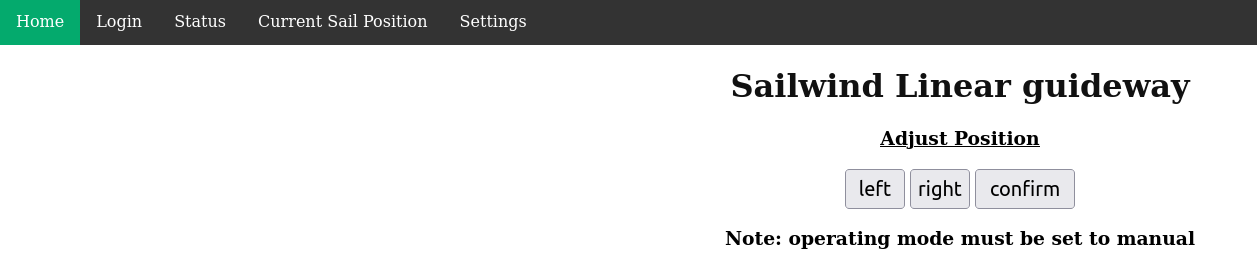
\includegraphics[width=\linewidth]{images/Software/Html_index_seite.png}
	\caption{Index Seite des Webservers}
	\label{fig:HTMLindex}
\end{figure}
\noindent Hier befindet sich die manuelle Steuerung zur Positionierung der Segel. Auf allen Seiten wird dabei am oberen Rand eine Navigations Bar angezeigt mit der zu den anderen Seiten Navigiert wird. Auf der Positionsdaten Seite ist der aktuelle Betriebsmodus und die Trimmung/Rollung der Segel zu finden. Die Sensordaten Seite zeigt alle aktuellen Werte der Sensoren an und wird regelmäßig aktualisiert. Die Einstellungsseite zeigt die aktuellen Einstellungen und macht es möglich den Betriebsmodus zu ändern, das Gerät neuzustarten und eine neue IP Adresse festzulegen oder \ac{DHCP} zu aktivieren. Die Login Seite hat aktuell keine Funktion und dient nur als Platzhalter. Hier könnten später je nach Nutzer die aufrufbaren Webseiten eingeschränkt werden. So kann z.B ein Service Mitarbeiter auf alle Einstellungen zugreifen, während ein normaler Nutzer nur z.B die Sensordaten abfragen kann. Die Error Seite wird nur bei einer Zeitüberschreitung der Anfrage angzeigt und hat keinen weiteren Nutzen.
\subsubsection{Umsetzung}
Die Webserver erhält dieselbe \ac{IP} Adresse wie die \ac{REST} \ac{API} ist aber auf dem Port 80 erreichbar. Im Gegensatz zum \ac{REST} interface bietet \ac{LWIP} hier bereits schon eine fertige Webserver implementierung. Dabei können Daten über die \ac{SSI} und \ac{CGI} Handler Übertragen werden. Beim Aufrufen einer Webseite werden die im \ac{HTML} Code festgelegten \ac{SSI} Tags mit den entsprechenden Sensor Daten oder Text mit einer Rückmeldung für den User ersetzt. Hierfür wurde ein zentrales \verb|switch-case| festgelegt, das nach der Nummer des \ac{SSI} Tags unterscheidet und den dementsprechend String einfügt. Der \ac{CGI} Handler wird für Textboxen oder für Buttons genutzt. Für Buttons wurden dafür \ac{HTML} Forms genutzt. Diese haben als \verb|Action| einen \ac{URI} wie in \autoref{lst:URI} zusehen ist. 
\begin{lstlisting}[language=C, caption={GET /data/adjustment Antwort Paket}, label={lst:URI}]
	<form action="/form_control.cgi">
	<p>
	<input type="submit" 
	id="move" 
	value="confirm" 
	name="move" 
	style="width:100px;height:40px;font-size:20px;">
	</p>
	</form>
\end{lstlisting}
Wird jetzt z.B auf der Index Seite der Button \glqq{}Confirm\grqq{} angeklickt wird der String: \verb|/form_control.cgi?move=confirm| zum Mikrocontroller gesendet. Auf Basis dieses String kann daraufhin eine Aktion gewählt werden und z.B die Anzeige auf dem Webserver verändert werden. Textinputs funktionieren ähnlich nur das sie den Inhalt der Textbox nach der \ac{URI} beinhalten.




